\documentclass[12p]{article}
\usepackage[utf8]{inputenc}

\usepackage{algorithm2e,algorithmic}
\usepackage{graphicx}
\usepackage{amsmath}
\usepackage{amsfonts}
\usepackage{enumitem}
\usepackage{multirow,array,varwidth}
\usepackage{booktabs}
\usepackage[round]{natbib}

%%%%%%%%%%%%%%%% Lengths %%%%%%%%%%%%%%%%
\setlength{\textwidth}{15.5cm}
\setlength{\evensidemargin}{0.5cm}
\setlength{\oddsidemargin}{0.5cm}

%%%%%%%%%%%%%%%% Variables %%%%%%%%%%%%%%%%
\def\titre{Studying and assisting the functional program design process.}

\begin{document}

%%%%%%%%%%%%%%%% Header %%%%%%%%%%%%%%%%
\fbox{
      {\itshape \titre}
}

%%%%%%%%%%%%%%%% Body %%%%%%%%%%%%%%%%
\section*{Context}

Functional programming is a domain of programming languages based on
lambda calculus. This mathematical abstraction can be shown to be
equivalent to combinatory logic. Consequently the programs written
with the functional paradigm can be proven more easily than with other
paradigms \citep{wadler_theorems_1989,voigtlander_proving_2008}. This
is a highly desirable property; it means that a program can be proven
to do what it is expected to. Functional programming, because of its
higher-order functions and lazy evaluation, also promotes software
modularity \citep{hughes_why_1989}, increasing the code readability
and reusability. This paradigm is more and more used in industry, but
unlike the object paradigm, for instance, it lacks a unified design
methodology to assist the software
development. \citet{russell_FAD_2001} tried to give the community a
tool similar to UML but dedicated to the functional paradigm. This
approach, however, seems not to have convinced the programmers. One
reason may be that it did not reflect the way they are used to
program. Another approach could be to investigate the methods used in
industry and use the results to develop a tool.\\

\section*{Objectives}
This PhD aims to understand how functional programmers develop their
software, with the intention to produce a unified methodology and an
adapted set of tools. An in-industry survey would give the PhD student
the possibility to assess the design process used by senior
programmers. Moreover the concept of unified methodology also needs to
be comprehensive with the current customs and what senior programmers
feel is effective or significant. This placement will also be the
opportunity to build a contact network, for the tools feedback later
in the PhD. Therefore there is a need to find a set of companies
willing to get involve in the project and ready to accept an intern to
collect data over the development. Prior to the industry survey, a
research protocol and a set of tools should be specified to help data
collection. Ideally, it would consist of the development of a ``black
box'' processing a source code using different metrics and saving the
measurements for later analysis. A set of benchmark programs, with
different complexities and aims, for instance a program needing 
particular attention to its extensibility, would help the comparison
between different representations. These few ideas could also be
completed by surveys and tools inspired by anthropological
studies. This preparation will allow for a systematic approach,
keeping track of the largest amount of data over the development
process. A brief study of the functional programming design process
revealed an important role played by refactoring. The goal of the
study would be to understand how it is used and possibly to represent
it in the methodology itself. More than representing the functional
paradigm, it should also represent the design process itself.\\

\section*{Approach}
The first part of the PhD would be dedicated to learn about tools used
in ethnographic studies, taking advantage of this social science in
the survey. The results obtained over the survey period used in
relation with software metrics should lead to a more robust and
automated tool. Some previous works on software metrics are promising
and can be applied to every paradigm. \citet{zimmermann_mining_2005}
offers an interesting approach by studying version manager history,it
gives a notion of code evolution and takes bug fixes into
consideration. This is, however, extremely dependent on how the
version manager is used. Later studies by
\citet{zimmermann_predicting_2008} and \citet{soliman_utilizing_2010}
based their approaches on dependency graphs and UML models. These
metrics can be applied even before any code is produced. They both
need a graphic model to be applied, therefore such a unified model
could help develop more metrics in functional programming. These
metrics intend to highlight the critical point of an application, a
high complexity being more likely to result in faults. Note that the
aim of these metrics is revealing the parts of the code that need to
be tested in depth or assigned to experienced
programmers. \citet{ryder_software_2005} studied several metrics in
the context of functional programming and mentioned the possibility of
using to use them to implement tools supporting the development in the
functional paradigm. The knowledge gained by the industry experience
could reveal new metrics, perhaps specific to the functional paradigm,
to be studied. The study of different metrics could be the opportunity
to write a review article on metrics applied to the functional
paradigm.

The second part, the investigation among industry programmers, should
collect data such as the represention used to keep track of the
different modules and their interactions. Moreover, studying the
reasons and criteria considered to choose a particular architecture
could lead to the definition of a set of metrics. Two approaches can
be considered with regards to the choice of companies. The first one
is to find an internship of 1 year in a company giving the opportunity
to follow a project over the long term, possibly from its beginning to
its end. The second is to find contacts in 3 or 4 companies in which
spending 3 to 4 months to have a better sampling over the different
methodologies. If the survey environment is detailed enough, it is
also possible to ask companies to fill the survey themselves, however
this would require a more significant effort on their part and is
therefore less likely to work. Depending on the results of the survey the
different customs observed in industry could lead to an article and
tentative unified methodology. The survey results may also lead to the
study of new metrics, which could be the opportunity of publishing
another article.

The third part will be dedicated to the development of a software tool
inspired and guided by the results of the survey. Frequent feedback
and user experiments should be used to drive its development
process. Such an approach ensures that the final tool meets the
expectation of current programmers. A wiki or a github repository
could be used to exchange with the community. At the end of second
year of the PhD organising a workshop may help finishing the
specification of the methodology and introduce a first version of the
developed software. This software will be released at the end of the
PhD and should help the development of functional applications.






\section*{Planning}

\begin{itemize}
\item[T1] the industry survey and its preparation
\item[T2] development of software metrics
\item[T3] survey result analysis and specification of a unified
  methodology
\item[T4] development, in relation with contacts in industry, of
  a tool inspired by the survey results and using the software metrics
  to diagnose the code
\item[T5] writing the PhD thesis
\end{itemize}


\begin{figure}[h]


\centering
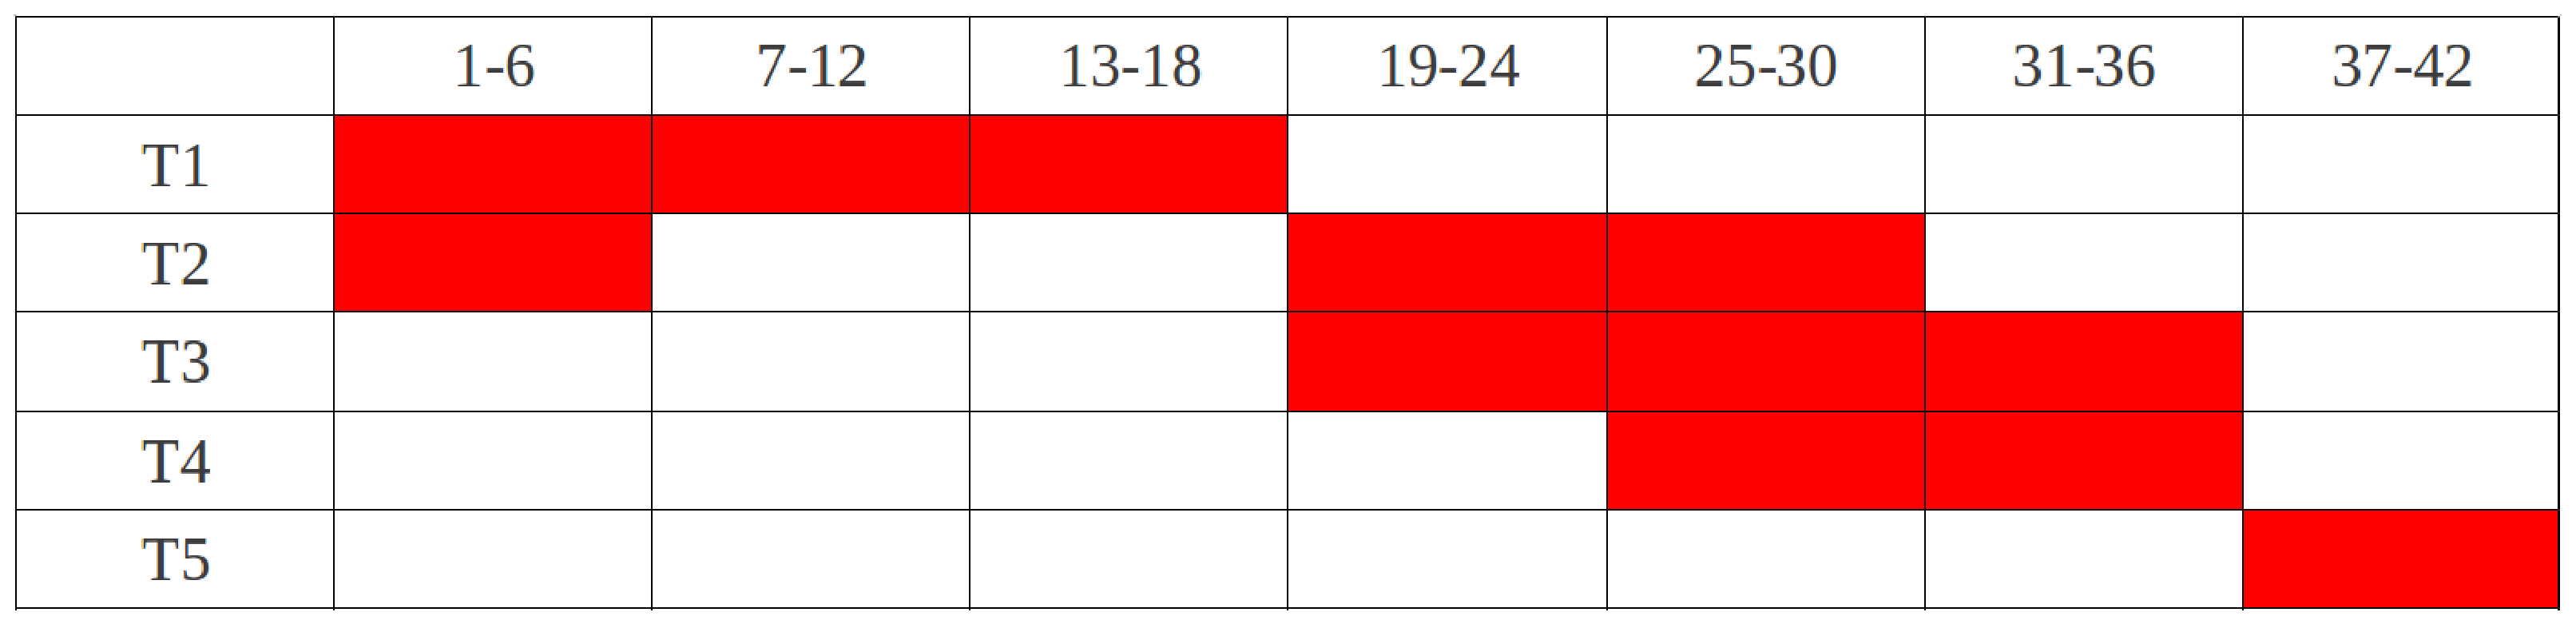
\includegraphics[width = 10cm]{planning.eps}
\caption{Planning of the different work packages, the columns represents the months.}
\label{fig:planning}
\end{figure}


\bibliographystyle{plainnat}
\bibliography{research-proposal}

\end{document}
